%%%%%%%%%%%%%%%Conjectures regarding values of Riemann zeta function at Gram points%%%%%%%%%%%%%%%%%%%%%%%%%%%%%%%%%%%%%%%%%%%%%%%%%%%%%%%%%%%%%
%

\documentclass[twoside]{article}
\usepackage{graphicx}
\usepackage{amsmath,amsthm,amssymb,verbatim}
\usepackage{fancyhdr}
\pagestyle{fancy}
\usepackage{url}
\usepackage{xcolor}


\def\blfootnote{\xdef\@thefnmark{}\@footnotetext} 
\long\def\symbolfootnote[#1]#2{\begingroup%
\def\thefootnote{\fnsymbol{footnote}}\footnote[#1]{#2}\endgroup} 

\newtheorem{mydef}{Conjecture}
\newtheorem*{mydef-non}{Conjecture}

\theoremstyle{definition}
\newtheorem{defn}{Definition}

\setcounter{page}{1}
\begin{document}

\date{}
\lhead[]{}
\chead[]{}
\rhead[]{}

\title{\bf{Symmetry properties of distribution of Riemann Zeta Function values on critical axis}}
%

\author{O. Shanker 
 \thanks{Mountain View, CA 94041, U. S. A. Email: oshanker@gmail.com
 }
}

\maketitle
\thispagestyle{fancy}

\begin{abstract}
In this work 
\end{abstract}

\symbolfootnote[0]{
\url{https://sites.google.com/site/riemannzetazeros/conjectures} 
}


%\clearpage
\chead[\underline{O. Shanker}]{\underline{Symmetry properties of distribution of Riemann Zeta Function values on critical axis}}


\section{Introduction}
The The paper is organized as follows.
Section~\ref{sec2} establishes the required notation for the 
Riemann Zeta Function. 
\section{\label{sec2}The Notation for the Riemann zeta function }

In this section we  establish the required notation for the 
Riemann Zeta Function. We follow closely the treatment in Ref.~\cite{Shanker 2018}.
For $\mathrm{Re} (s) > 1$ the Riemann Zeta function is defined as
\begin{equation}
\zeta ( s ) \, = \, \sum^{\infty}_{n = 1} \; n^{-s} \, = \, \prod_{p \in primes} \;
\left( 1 - p^{-s} \right)^{-1}.
\label{eqRie}
\end{equation}
 $\zeta ( s )$ can be continued to
the complex plane. It satisfies the functional equation \cite{Riemann(1858),Riemann 1892, Titchmarsh 1986,Edwards(1974)}
\begin{equation}  
\xi(s):=s(s-1) \pi^{-s/2} \, \Gamma (s/2) \, \zeta ( s )/2 \, = \, \xi ( 1 - s );
\label{eq:xifunc}
\end{equation}
$\xi(s)$ is an entire function. The zeroes of $\xi(s)$ are denoted by $1/2 + i \gamma$. The Riemann Hypothesis  
is that $\gamma$ is real for the non-trivial zeroes.
The $\gamma$s are ordered in increasing order, with 
\begin{equation}
\ldots \ldots \gamma_{-1} \, < \, 0 \, < \, 
\gamma_1 \, \leq \, \gamma_2 \ldots. 
\end{equation}
Then $\gamma_j \, = \, - \gamma_{-j}$ for $j = 1, 2, \ldots,$ 
and    $\gamma_1$, $\gamma_2$, $\ldots$  are roughly
$14.1347$, $21.0220$, $\ldots$.

Asymptotically, the mean number of 
zeros for the Riemann zeta function with height less than $t$ (the smoothed Riemann zeta staircase, denoted by 
$N_{smooth}(t)$) is~\cite{Edwards(1974)}
\begin{equation}  
N_{smooth}(t) = (t/2\pi)(\ln(t/2\pi)-1)+\frac{7}{8}.
\label{eq:Rnumber}
\end{equation}
Thus, the mean spacing $\delta$ of the zeros at height $t$ is 
\begin{equation}  
\delta = 2\pi(\ln (t/2\pi))^{-1}. 
\label{eq:spacing}
\end{equation}
One defines
\begin{equation}
\theta(t) = arg (\pi^{it/2} \Gamma(\frac{1}{4} + \frac{it}{2})), 
\label{eq:theta}
\end{equation}
where the argument is defined by continuous variation of $t$ starting with the value $0$ at $t = 0$.
For large $t$, $\theta$ has the asymptotic expansion
\begin{equation}
\theta(t) \approx \frac{t}{2}\ln (\frac{t}{2\pi}) - \frac{t}{2} - \frac{\pi}{8} + \frac{1}{48t} - \frac{1}{5760t^3}. 
\label{eq:thetaAsymptotic}
\end{equation}
From the zeta functional equation it follows that Hardy's function 
\begin{equation}
Z(t)=exp(i\theta(t))\zeta(1/2 +it) 
\label{eq:hardy}
\end{equation}
is real valued for real $t$. 
Moreover we have $|Z(t)| = |\zeta(1/2+it)|$. Thus the zeros of $Z(t)$ are the imaginary part of the zeros 
of $\zeta(s)$ which lie on the critical line.  

Many of the zeros are separated by the
Gram points~\cite{Gram 1903}.  When $t \ge 7$, the $\theta$ function Eq.(\ref{eq:theta}) is monotonic increasing. 
\begin{defn}\label{gram}
For $n \ge -1$, the $n$-th Gram point $g_n$ is defined as the unique solution $> 7$ to
$\theta (g_n) = n\pi$. We call the Gram point an odd Gram point if $n$ is odd, and an even Gram point if $n$ is even.
A Gram interval is the interval $G_n = [g_n,g_{n+1})$.
\end{defn}
Thus, at a Gram point we have
\begin{equation}
\zeta(1/2+ig_n) = (-1)^{n}Z(g_n).
\label{eq:zetagram}
\end{equation}
Ref.~\cite{Shanker 2018} studied empirically the distribution of $Z(t)$ values at Gram points. We will generalize the study to other points on
the critical axis, as defined below. In analogy with Gram points, we can associate an angle $\phi$ with a point $t$ on the critical axis as follows:
\begin{defn}\label{phi}
For $t \ge 7$, $t$ is said to be a phi point if
$\theta (t) = 2k\pi + \phi$, where $0 \le \phi < 2\pi$.
\end{defn}
We will study the distribution of $Z(t)$ values at a given value of $\phi$, and investigate symmetry and anti-symmetry relations for the 
distributions at different values of $\phi$. Formally, our sample space is defined by
\begin{defn}\label{samplespace}The sample space for all the distributions in this work is an interval  at height $t$ which is large compared to the Gram interval, but small enough that we can consider {$\ln (t)$} to be essentially constant over the interval. 
\end{defn}
The notation $\ln (t)$ stands for the natural logarithm of $t$.  We define $p_{\phi}(y)$, the probability distribution function for $Z(t)$ at phi points:
\begin{defn}\label{pphi}
\begin{equation}
\int\limits_{a}^{b} p_{\phi}(y)dy
\label{eq:pdfphi}
\end{equation}
is the probability that $a<Z(t)<b$ when we consider the values of $Z(t)$ for a large number of phi points in the sample space. 
\end{defn}
In Ref.~\cite{Shanker 2018}  we defined
\begin{defn}\label{podd}
\begin{equation}
\int\limits_{a}^{b} p_{odd}(y)dy
\label{eq:pdfodd}
\end{equation}
is the probability that $a<Z(t)<b$ when we consider the values of $Z(t)$ for a large number of odd Gram points in the sample space. 
\end{defn}
$p_{even}(y)$ was defined analogously. In terms of Definition~\ref{pphi} we have $p_{odd}(y) = p_{\pi}(y)$ and $p_{even}(y) = p_{0}(y)$.
The probability densities $p_{odd}(y)$,  $p_{\phi}(y)$ and $p_{even}(y)$ depend on the sample space (i.e., on the height $t$ and on the size of the sample space). In practice the densities are not sensitive to the choice of the sample space as long as the height $t$ is large enough and the length of the interval from which the sample is collected is large enough (but not too large on log scale).

Ref.~\cite{Shanker 2018} conjectured that $p_{odd}(y) = p_{even}(-y)$. We generalize the conjecture as stated in Equations \ref{eq:mean}, \ref{eq:antisym} and \ref{eq:sym} below.
The mean value $\langle Z(t_{\phi})\rangle$ is given by
\begin{equation}
\langle Z(t_{\phi})\rangle = 2\cos (\phi).
\label{eq:mean}
\end{equation}
Equation \ref{eq:mean} was explicitly called out for Gram points in Ref.~\cite{Titchmarsh 1986}. Empirically, we find that $p_{\phi}(y)$ satisfies the conditions
\begin{equation}
p_{\phi}(y) = p_{\phi+\pi}(-y),
\label{eq:antisym}
\end{equation}
and
\begin{equation}
p_{\phi}(y) = p_{2\pi-\phi}(y).
\label{eq:sym}
\end{equation}
The empirical evidence for these generalizations is given in the next section.


\begin{figure*}
\centering
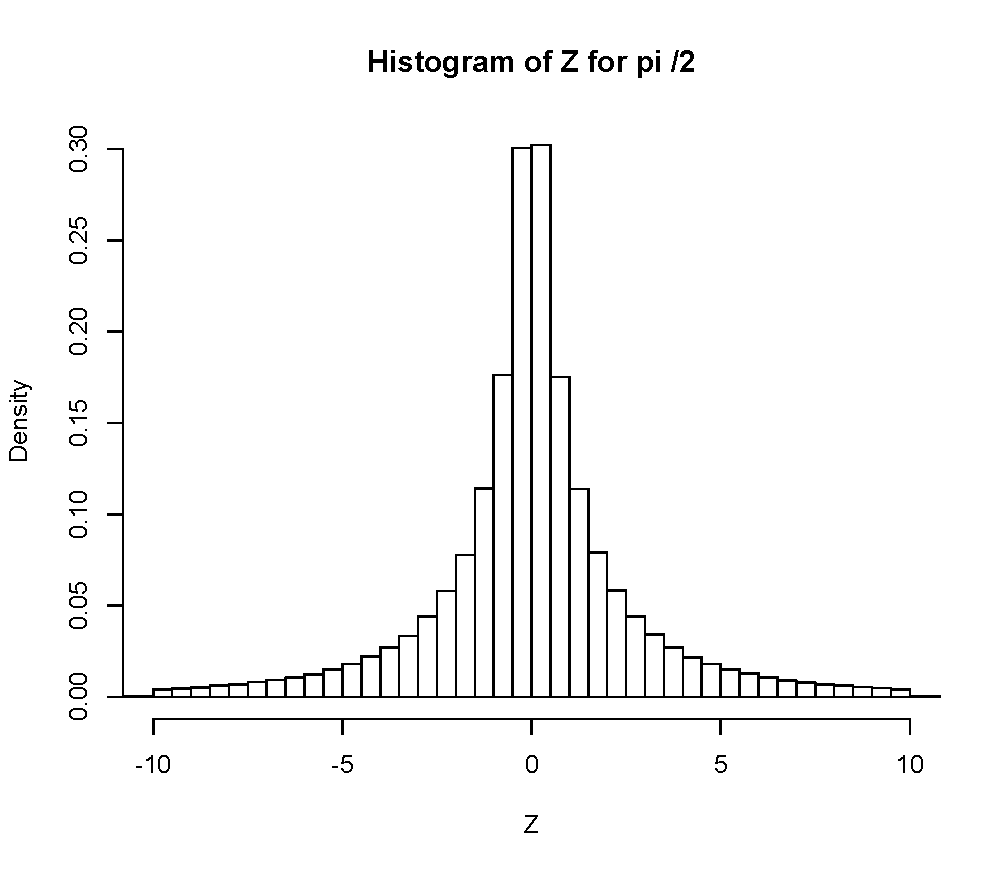
\includegraphics[width=0.8\textwidth]{pi2plot.pdf}
\caption[]{ 
 Distribution of zeta values at $\phi = \pi/2$.
  }
\vspace{1mm}
\label{pi2}
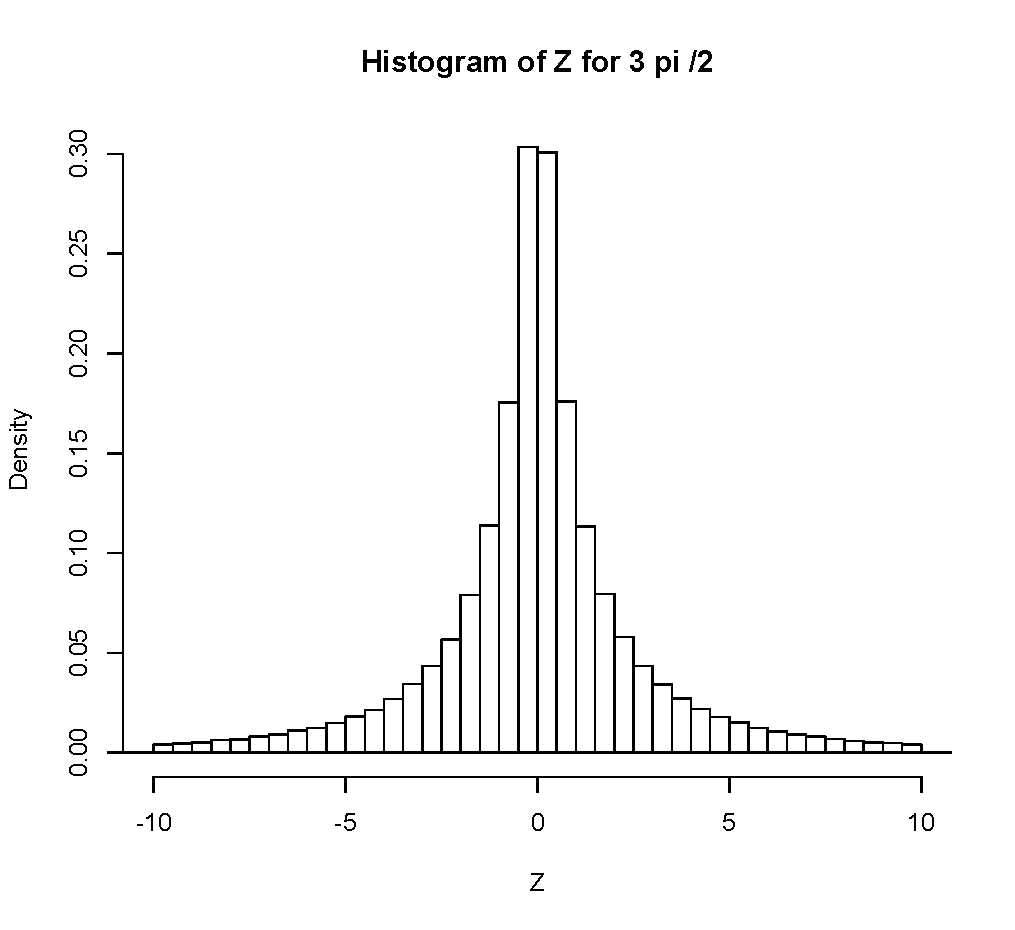
\includegraphics[width=0.8\textwidth]{3pi2plot.pdf}
\caption[]{ 
 Distribution of zeta values at $\phi = 3\pi/2$.
  }
\vspace{1mm}
\label{3pi2}
\end{figure*}



\section{\label{sec7}Symmetry relations}


\begin{table}
\centering \(\begin{array}{ccccccc}
\hline
 \phi &     Min.   & 1st    &  Median    &   Mean   & 3rd    &   Max. \\
 &              & Quantile   &            &              & Quantile.    &   \\
\hline
0 &-69 &0.1134 &0.8517 &2.0001 &2.5403 &165  \\
1 &-97 &-0.1352 &0.5916 &1.4143 &2.1226 &159 \\
2 &-121 &-1.082 &0.0017 &0.0001 &1.089 &137 \\
3 &-148 &-2.1121 &-0.5852 &-1.4141 &0.1364 &103 \\
4 &-161 &-2.5277 &-0.8467 &-1.9999 &-0.1122 &69 \\
5 &-153 &-2.1045 &-0.5891 &-1.4141 &0.1365 &105 \\
6 &-129 &-1.083 &-0.001 &0.0001 &1.084 &138 \\
7 &-93 &-0.1336 &0.5883 &1.4143 &2.1077 &160 \\
\hline
\end{array}\)
\caption{Quantiles and mean for  $Z(t)$ at Gram points of different types.} 
\label{tab:quantiles}
\end{table}


\begin{table}
\centering \(\begin{array}{ccccccc}
\hline
 \phi &     Min.   & 1st    &  Median    &   Mean   & 3rd    &   Max. \\
  &              & Quantile   &            &              & Quantile.    &   \\
\hline
0 & -69 & 0.1134 & 0.8517 & 2.0001 & 2.5403 & 165 \\
1 & -88 & 0.0167 & 0.7318 & 1.7321 & 2.3515 & 162\\
2 & -105 & -0.3877 & 0.4108 & 1.0001 & 1.8151 & 154\\
3 & -121 & -1.082 & 0.0017 & 0.0001 & 1.0888 & 137\\
4 & -140 & -1.81 & -0.4053 & -0.9999 & 0.3904 & 115 \\
5 & -155 & -2.338 & -0.7258 & -1.732 & -0.0160 & 91\\
6 & -161 & -2.5277 & -0.8467 & -1.9999 & -0.1122 & 69\\
7 & -158 & -2.334 & -0.7294 & -1.732 & -0.0161 & 93\\
8 & -147 & -1.8034 & -0.4097 & -0.9999 & 0.388 & 117\\
9 & -129 & -1.083 & -0.001 & 0.0001 & 1.0842 & 138\\
10 & -105 & -0.3855 & 0.4086 & 1.0001 & 1.8103 & 154\\
11 & -80 & 0.0184 & 0.7317 & 1.7322 & 2.3393 & 164 \\
\hline
\end{array}\)
\caption{Quantiles and mean for  $Z(t)$ at Gram points of different types.}
\label{tab:quantiles6}
\end{table}

Table~\ref{tab:quantiles} shows the quantiles and mean for  $Z(t)$ a.  Table~\ref{tab:quantiles6} shows the quantiles and mean for  $Z(t)$ a. The statistics are from $1$ million Gram intervals at $t=10^{12}$. Fig.~\ref{pi2} Fig.~\ref{3pi2}
\section{\label{conclusions}Conclusions}

In this work 
\begin{thebibliography} {}

\bibitem{Shanker 2018} O. Shanker, 
``Good to Bad Gram Point Ratio For Riemann Zeta Function",
{\it Experimental Mathematics} {\bf doi:10.1080/10586458.2018.1492474}(2018)



\bibitem {Riemann(1858)} B. Riemann, ``\"{U}ber die Anzahl der Primzahlen uter
Einer Gegebenen Gr\"{o}be,'' {\it Montasb. der Berliner Akad.}, (1858),
671-680

\bibitem {Riemann 1892} B. Riemann, ``Gesammelte Werke'', Teubner, Leipzig, (1892)

\bibitem {Titchmarsh 1986} E. Titchmarsh, ``The Theory of the Riemann Zeta
Function,'' Oxford University Press, Second Edition, (1986)

\bibitem {Edwards(1974)} H. M. Edwards, ``Riemann's Zeta Function,''
Academic Press,  (1974)

\bibitem{Gram 1903} J. P. Gram, 
``Sur les Zeros de la Fonction  $\zeta ( s )$  de Riemann",
{\it Acta Math.} {\bf27}(1903), 289-304


\end{thebibliography} 

\end{document} 
